\section{Method: PCU-Select}
\label{sec:method}

PCU-Select learns the conditional utility surrogate in Eq.~\eqref{eq:surrogate} and selects a budgeted subset for a target PEFT--task pair. Figure~\ref{fig:architecture} summarizes two stages. Offline, it extracts reusable sample and task signals, constructs two types of utility label, and trains one scorer. Online, it combines cached sample features with a target $(p^{*},t^{*})$, scores the pool, and distributes budget across semantic clusters. Supplementary Algorithms~S1 and~S2 specify both stages.

\begin{figure*}[t]
\centering
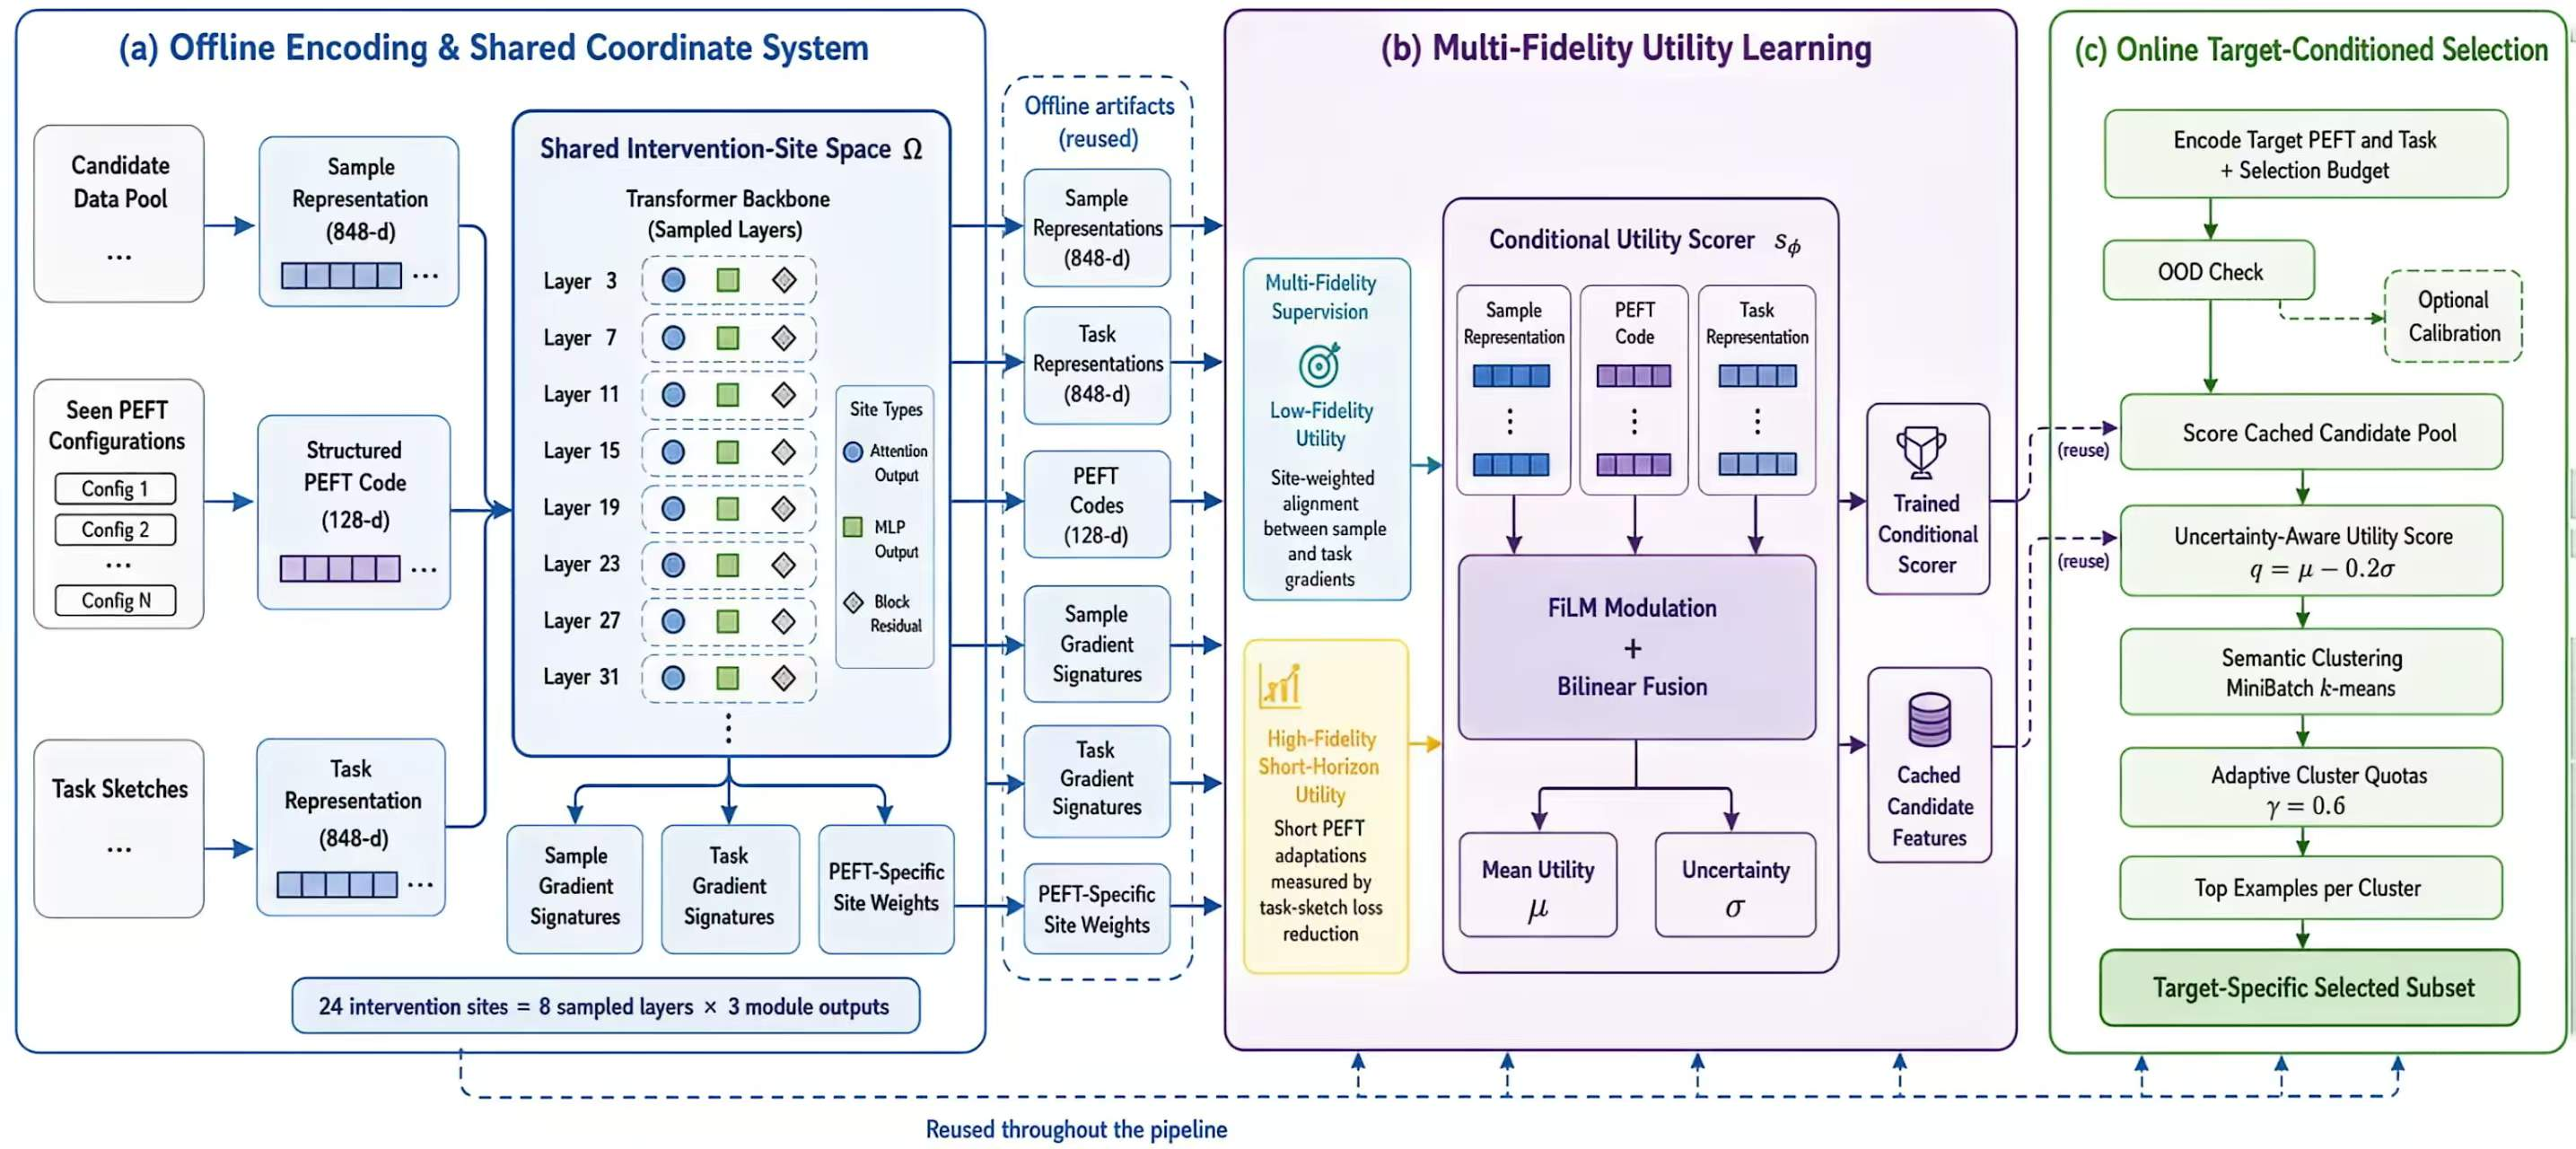
\includegraphics[width=\textwidth]{Figures/image.jpg}
\caption{PCU-Select learns from reusable site-level signals and scores each PEFT--task target online. A 24-site coordinate system aligns sample and task gradients with a 128-dimensional structured PEFT code; proxy and short-update labels provide complementary supervision.}
\label{fig:architecture}
\end{figure*}

\subsection{Shared Intervention Sites Enable Cross-PEFT Reuse}

PEFT families expose parameter tensors with different shapes and roles, so their raw gradients cannot share one cache~\cite{hu2022lora,houlsby2019adapters,liu2022ia3}. PCU-Select instead uses a fixed set $\Omega$ of \emph{intervention sites}. Each site is a selected module output through which a PEFT update affects the backbone. The set $\Omega$ is a shared coordinate system because sample gradients, task gradients, and each PEFT's map of affected sites all use the same index $\omega$.

PCU-Select hooks attention, MLP, and post-residual outputs at eight evenly spaced Transformer layers, giving $|\Omega|=24$. A site's response-loss gradient describes how a sample or task pushes that activation. By the chain rule, PEFT-parameter gradients factor through gradients at the module outputs they modify. Site gradients therefore avoid both full PEFT-parameter reconstruction and shape mismatches between fused and split projections. Post-residual sites place adapters in the same index space as LoRA and (IA)$^3$.

A site index records only \emph{where} a configuration acts. PCU-Select separately encodes operator and capacity features to record \emph{how} it acts and how much it can update. This factorization reuses one sample signature without treating additive, multiplicative, and bottleneck updates as equivalent.

Each configuration maps to a site mask and operator type. Attention LoRA and (IA)$^3$-attention map to attention-output sites. MLP LoRA and (IA)$^3$-FFN map to MLP-output sites, while adapters map to block-residual sites. Prefix tuning maps to attention-output sites. LN Tuning updates Llama-2's per-block RMSNorm scales~\cite{wang2022lntuning,touvron2023llama2}: input-normalization scales map to attention-output sites, and post-attention-normalization scales map to MLP-output sites. The configuration excludes the final model-level RMSNorm. Both site types use the multiplicative operator channel. These mappings define each normalized site weight:
\begin{equation}
  \begin{aligned}
  w_p^{\omega}
  &=\mathrm{mask}(p,\omega)\,\kappa(p,\omega),\\
  \kappa(p,\omega)
  &=\tanh\!\left(\eta\log(1+\mathrm{cap}(p,\omega)/d_{\mathrm{model}})\right),\\
  \tilde{w}_p^{\omega}
  &=w_p^{\omega}/\max(\varepsilon_w,\sum_{\omega'}w_p^{\omega'}).
  \end{aligned}
  \label{eq:site-weight}
\end{equation}
Here $\mathrm{mask}(p,\omega)$ is zero at untouched sites, and $\mathrm{cap}(p,\omega)$ measures trainable capacity. The width $d_{\mathrm{model}}$ normalizes capacity, $\eta$ controls saturation through $\tanh$, and $\varepsilon_w$ keeps the denominator nonzero. Thus, $\tilde{w}_p^{\omega}$ distributes unit weight over the sites used by $p$. Supplementary Table~S8 maps LoRA rank, adapter width, (IA)$^3$ vector count, prefix length, and LN-Tuning scale count to this quantity. Operator type remains separate in $z_p$ because a family-wide scalar would cancel under Eq.~\eqref{eq:site-weight}'s normalization.

\subsection{Shared Representations Preserve Target Specificity}

Shared site indices make signals comparable, but the scorer must still distinguish each sample, task, and PEFT. PCU-Select uses three fixed-length vectors: the sample representation describes the example, the task representation describes the target need, and the PEFT representation describes where and how training acts. Site gradients supply separate label-construction signals.

The sample representation $z_x=[e_x;d_x;a_x]\in\mathbb{R}^{848}$ combines semantic, descriptive, and activation features. The 768-dimensional $e_x$ is the frozen \texttt{sentence-transformers/all-mpnet-base-v2} embedding of the instruction and response~\cite{song2020mpnet,reimers2019sentencebert}. This encoder remains frozen during pool and target-benchmark processing. The 16-dimensional $d_x$ records length, response-LM loss, entropy, and format. The 64-dimensional $a_x$ summarizes response-token hidden states at the eight sampled layers.

Utility is task-relative, so PCU-Select forms $z_t\in\mathbb{R}^{848}$ by mean-pooling $z_x$ over the task sketch's 32 examples. For proxy labels, it separately averages their site gradients into $g_t^{\omega}$. These $24\times256$ values remain outside $z_t$ and serve only label construction.

The PEFT representation records the target trainable subspace. In $z_p=[m_p;c_p;r_p]\in\mathbb{R}^{128}$, the $24\times4$ mask $m_p$ contributes 96 dimensions. Its channels mark active sites, additive updates, multiplicative scaling, and prefix-style control. Two 16-dimensional vectors encode capacity $c_p$ and training recipe $r_p$. At this site resolution, q/v and q/k/v/o LoRA share attention-output sites, while capacity and recipe preserve their projection-level distinction.

Prefix, P-Tuning, and LN Tuning use the same deterministic encoding rules as seen families. The scorer has no learned family lookup or operator centroid. The support policy below decides whether a target uses direct scoring, calibrated scoring, or a per-target selector.

Training these representations requires labels for many $(x,p,t)$ triples, but measuring every PEFT update would defeat amortization. PCU-Select instead uses \emph{multi-fidelity supervision}, which combines labels with different costs and directness. A low-fidelity gradient proxy cheaply covers the pool. High-fidelity short updates directly measure sketch-loss reduction for fewer triples. Together, they learn broad ranking structure and correct errors near the subset cutoff.

The \emph{gradient-proxy label} measures alignment between a sample and the task sketch at sites used by the target PEFT:
\begin{equation}
  u^{\mathrm{lo}}(x,p,t)=\sum_{\omega\in\Omega}\tilde{w}_p^{\omega}
  \cos\!\left(g_x^{\omega},g_t^{\omega}\right).
  \label{eq:ulo}
\end{equation}
Here $g_x^{\omega}$ is the response-token loss gradient at site $\omega$. A Johnson--Lindenstrauss random projection~\cite{johnson1984jl} compresses it to 256 dimensions and unit-normalizes the result. The task-sketch mean gives $g_t^{\omega}$. Equation~\eqref{eq:ulo} therefore measures alignment only at sites used by $p$. All sketches use response-token cross-entropy for these signatures; task-native metrics such as option likelihood, Pass@1, and F1 remain downstream evaluation metrics. Because cosine values can be negative, PCU-Select rank-normalizes them within each $(p,t)$ bucket before proxy distillation and ranking. Cached sample signatures then label many $(x,p,t)$ triples without new gradient extraction.

The \emph{short-update label} measures realized sketch-loss reduction near the subset cutoff. For each sampled triple, PCU-Select uses two anchors $\theta_a$: the base model and a warm checkpoint after adaptation has begun. The horizon $h$ is the number of short-update steps. A mini-batch $\mathcal{B}(x)$ contains the sampled example and seven condition-matched fillers. PCU-Select applies PEFT $p$ for $h$ steps and measures
\begin{equation}
  \Delta(x,p,t,a,h)=L_{V_t}(\theta_a)-
  L_{V_t}\!\left(\mathrm{Adapt}^{h}_{p}(\mathcal{B}(x);\theta_a)\right).
  \label{eq:delta}
\end{equation}
Thus, $\Delta$ is the task-sketch loss before the update minus its loss afterward. Rank-normalized reductions for $h\in\{1,4\}$ from both anchors define $u^{\mathrm{hi}}$. The fillers make this mini-batch effect more stable than a single-example update. PCU-Select allocates 10K short-update labels in three stages. Coverage sampling first spreads labels across the registry without a scorer.

Coverage labels and the proxy then train a provisional scorer. It predicts ranks and a per-triple uncertainty scale, an estimate of prediction noise. Uncertainty sampling selects triples with large scales. Boundary sampling selects large predicted--observed rank disagreements near the cutoff. Every rank normalization compares labels within one PEFT, task, anchor, and horizon bucket.

The proxy cheaply orders the full pool, while short updates target consequential ranking errors. Two anchors test whether utility persists after adaptation begins; two horizons reduce dependence on one update length. Ranking within condition-matched buckets avoids assuming a shared raw-loss scale across tasks or configurations.

\subsection{Conditional Scoring Produces Target-Specific Subsets}

The scorer consumes $(z_x,z_p,z_t)$ and predicts $(\hat{\mu},\hat{\sigma})=s_{\phi}(z_x,z_p,z_t)$. Here $\hat{\mu}$ gives predicted mean utility, while $\hat{\sigma}$ gives a positive, input-dependent uncertainty scale. Separate encoders map the three inputs into hidden vectors. FiLM modulation~\cite{perez2018film} uses the PEFT and task codes to rescale and shift sample features. A bilinear term represents sample--PEFT compatibility.

Stage A distills gradient-proxy ranks to learn broad conditional structure. Stage B continues proxy distillation and adds ranking and regression on short-update labels plus a heteroscedastic uncertainty loss. Here \emph{heteroscedastic} means that predicted noise can differ across triples. PCU-Select selects the Stage B checkpoint on held-out PEFT--task pairs. It also fixes the sketch size, label allocation, anchors, horizons, and scalar selection hyperparameters on these pairs before downstream evaluation.

A target's structural support level determines whether PCU-Select applies the scorer directly or calibrates it. Relative to the seen registry, L0 resembles a seen configuration, L1 makes a larger shift within a seen family, and L2 introduces an unseen family. Seen targets use the trained scorer directly. L0 targets run \emph{zero-shot}: PCU-Select scores a new configuration without target-specific short-update labels. L1 and L2 targets use calibrated scoring when compatible labels exist and a per-target selector otherwise.

After any required calibration, PCU-Select converts the two scorer outputs into a conservative ranking score:
\begin{equation}
  q(x)=\hat{\mu}(x,p^{*},t^{*})-\lambda\hat{\sigma}(x,p^{*},t^{*}),\qquad \lambda=0.2.
  \label{eq:qscore}
\end{equation}
The uncertainty scale reduces the rank of examples whose predicted utility is noisy. It serves as a ranking penalty, not a confidence interval.

Ranking by $q$ alone can over-select near-duplicates, so PCU-Select clusters examples in semantic space before assigning the budget. It allocates budget $B$ across $K$ clusters $C_k$, where $k\in\{1,\ldots,K\}$:
\begin{equation}
  b_k=\mathrm{round}\!\left(
  B\frac{(v_k^{+})^{\gamma}|C_k|^{1-\gamma}}
  {\sum_j(v_j^{+})^{\gamma}|C_j|^{1-\gamma}}\right),\qquad \gamma=0.6.
  \label{eq:quota}
\end{equation}
Here $v_k$ is the mean conservative score among the top 10\% of examples in $C_k$, and $v_k^{+}=\max(v_k,0)$. The factors $v_k^{+}$ and $|C_k|$ balance cluster value and size. For the 300K pool, $K=\max(50,\lfloor\sqrt{N}\rfloor)$ produces 547 clusters of about 548 examples. The reported end-to-end cost is 0.38 GPU-hours per PEFT--task application and includes clustering. PCU-Select takes the top-$b_k$ examples by $q$ within each cluster. Non-positive clusters receive no budget; deterministic remainder handling makes the quotas sum to $B$.

For seen and L0 targets, all gradient extraction and label construction occur offline; online selection uses cached features and scorer forward passes. L1 and calibratable L2 targets add a small label set without rebuilding a target-specific gradient datastore. The evaluation next tests whether this reuse preserves LESS-level quality, reduces registry cost, and transfers across support levels.
